%% March 2018
%%%%%%%%%%%%%%%%%%%%%%%%%%%%%%%%%%%%%%%%%%%%%%%%%%%%%%%%%%%%%%%%%%%%%%%%%%%%
% AGUJournalTemplate.tex: this template file is for articles formatted with LaTeX
%
% This file includes commands and instructions
% given in the order necessary to produce a final output that will
% satisfy AGU requirements, including customized APA reference formatting.
%
% You may copy this file and give it your
% article name, and enter your text.
%
%
% Step 1: Set the \documentclass
%
% There are two options for article format:
%
% PLEASE USE THE DRAFT OPTION TO SUBMIT YOUR PAPERS.
% The draft option produces double spaced output.
%

%% To submit your paper:
\documentclass[draft]{agujournal2018}

\usepackage{amsmath}
\usepackage{amssymb}

\usepackage{apacite}
\usepackage{url} %this package should fix any errors with URLs in refs.
\usepackage{lineno}
\linenumbers
%%%%%%%
% As of 2018 we recommend use of the TrackChanges package to mark revisions.
% The trackchanges package adds five new LaTeX commands:
%
%  \note[editor]{The note}
%  \annote[editor]{Text to annotate}{The note}
%  \add[editor]{Text to add}
%  \remove[editor]{Text to remove}
%  \change[editor]{Text to remove}{Text to add}
%
% complete documentation is here: http://trackchanges.sourceforge.net/
%%%%%%%

\draftfalse

%% Enter journal name below.
%% Choose from this list of Journals:
%
% JGR: Atmospheres
% JGR: Biogeosciences
% JGR: Earth Surface
% JGR: Oceans
% JGR: Planets
% JGR: Solid Earth
% JGR: Space Physics
% Global Biogeochemical Cycles
% Geophysical Research Letters
% Paleoceanography and Paleoclimatology
% Radio Science
% Reviews of Geophysics
% Tectonics
% Space Weather
% Water Resources Research
% Geochemistry, Geophysics, Geosystems
% Journal of Advances in Modeling Earth Systems (JAMES)
% Earth's Future
% Earth and Space Science
% Geohealth
%
% ie, \journalname{Water Resources Research}

\journalname{Enter journal name here}


\begin{document}

%% ------------------------------------------------------------------------ %%
%  Title
%
% (A title should be specific, informative, and brief. Use
% abbreviations only if they are defined in the abstract. Titles that
% start with general keywords then specific terms are optimized in
% searches)
%
%% ------------------------------------------------------------------------ %%

% Example: \title{This is a test title}

\title{=enter title here=}

%% ------------------------------------------------------------------------ %%
%
%  AUTHORS AND AFFILIATIONS
%
%% ------------------------------------------------------------------------ %%

% Authors are individuals who have significantly contributed to the
% research and preparation of the article. Group authors are allowed, if
% each author in the group is separately identified in an appendix.)

% List authors by first name or initial followed by last name and
% separated by commas. Use \affil{} to number affiliations, and
% \thanks{} for author notes.
% Additional author notes should be indicated with \thanks{} (for
% example, for current addresses).

% Example: \authors{A. B. Author\affil{1}\thanks{Current address, Antartica}, B. C. Author\affil{2,3}, and D. E.
% Author\affil{3,4}\thanks{Also funded by Monsanto.}}

\authors{=list all authors here=}


% \affiliation{1}{First Affiliation}
% \affiliation{2}{Second Affiliation}
% \affiliation{3}{Third Affiliation}
% \affiliation{4}{Fourth Affiliation}

\affiliation{=number=}{=Affiliation Address=}
%(repeat as many times as is necessary)

%% Corresponding Author:
% Corresponding author mailing address and e-mail address:

% (include name and email addresses of the corresponding author.  More
% than one corresponding author is allowed in this LaTeX file and for
% publication; but only one corresponding author is allowed in our
% editorial system.)

% Example: \correspondingauthor{First and Last Name}{email@address.edu}

\correspondingauthor{=name=}{=email address=}

%% Keypoints, final entry on title page.

%  List up to three key points (at least one is required)
%  Key Points summarize the main points and conclusions of the article
%  Each must be 100 characters or less with no special characters or punctuation

% Example:
% \begin{keypoints}
% \item	List up to three key points (at least one is required)
% \item	Key Points summarize the main points and conclusions of the article
% \item	Each must be 100 characters or less with no special characters or punctuation
% \end{keypoints}

\begin{keypoints}
\item enter point 1 here
\item enter point 2 here
\item enter point 3 here
\end{keypoints}

%% ------------------------------------------------------------------------ %%
%
%  ABSTRACT
%
% A good abstract will begin with a short description of the problem
% being addressed, briefly describe the new data or analyses, then
% briefly states the main conclusion(s) and how they are supported and
% uncertainties.
%% ------------------------------------------------------------------------ %%

%% \begin{abstract} starts the second page

\begin{abstract}
enter abstract here

\end{abstract}



%% ------------------------------------------------------------------------ %%
%
%  TEXT
%
%% ------------------------------------------------------------------------ %%

%%% Suggested section heads:
% \section{Introduction}
%
% The main text should start with an introduction. Except for short
% manuscripts (such as comments and replies), the text should be divided
% into sections, each with its own heading.

% Headings should be sentence fragments and do not begin with a
% lowercase letter or number. Examples of good headings are:

% \section{Materials and Methods}
% Here is text on Materials and Methods.
%
% \subsection{A descriptive heading about methods}
% More about Methods.
%
% \section{Data} (Or section title might be a descriptive heading about data)
%
% \section{Results} (Or section title might be a descriptive heading about the
% results)
%
% \section{Conclusions}


\section{Introduction}

The largest earthquakes on Earth occur in subduction zones, where large segments of the boundary between the subducting tectonic plate and the overlying plate can store energy for centuries and then release it in minutes during an earthquake. To better assess seismic hazard, it is thus necessary to improve our understanding of subduction zone processes. Slow slip events are a new feature discovered in the last two decades in many subduction zones thanks to recordings of the displacement of Earth's surface by dense Global Navigation Satellite System (GNSS) networks. Slow slip events can last from a few days to several years, and have a relatively short recurrence time (months to years), compared to the recurrence time of regular earthquakes (up to several hundreds of years), allowing scientists to observe and study many complete event cycles, which is typically not possible to explore with traditional earthquake catalogs (Beroza and Ide, 2011 ~\cite{BER_2011}).  Moreover, whereas regular earthquakes occur in the seismogenic / locked zone, slow slip events occur downdip of the locked section of the subduction zone. Interactions between the slow slip zone and the seismogenic zone could potentially trigger large earthquakes. Through future study, this interaction may improve our understanding of the seismic hazard.

Wavelets methods such as the Discrete Wavelet Transform (DWT) are mathematical tools for analyzing time series simultaneously in the time and the frequency domain by observing how weighted averages of a time series vary from one averaging period to the next. They have been widely used for geophysical applications. However, very few studies have used wavelet methods to analyze recordings of slow slip events. The aim of this project is thus to use \textbf{wavelet methods to analyze GNSS recordings of slow slip events in Cascadia  and New Zealand}. These advanced signal processing methods will enable extracting much more information from the GNSS data currently available and will improve our knowledge of this newly discovered geological phenomenon. Specifically, as a result of the project, I will be able to \emph{detect possible smaller (magnitude 5) slow slip events} in Zealand that may be currently undetected with standard methods and \emph{detect longer (months to years) slow slip events} that are more difficult to detect than slow slip events with a short duration (days to weeks). Additionally, the methods developed for the study of slow slip events can have a broader potential impact for the detection of transient signals in GNSS time series. The codes developed will be publicly released on the student's GitHub repository (url available on the student's CV). 

\textbf{2. Introduction}

As with ordinary earthquakes, slow slip events are caused by slip on a fault, such as the plate boundary between a tectonic plate subducting under another tectonic plate. However, they take a much longer time (several days to several years) to happen relative to ordinary earthquakes. Moreover, the seismic waves they generate are much weaker than the seismic waves generated by ordinary earthquakes, and may not be detectable.  A slow slip event on the plate boundary is inferred to happen when there is a reversal of the direction of motion at GNSS stations, compared to the secular interseismic motion. Slow slip events have been observed in many subduction zones, such as Cascadia, Nankai (southwest Japan), Alaska, Costa Rica, Mexico, and New Zealand (Beroza and Ide, 2011 ~\cite{BER_2011}; Audet and Kim, 2016 ~\cite{AUD_2016}).

In many places, tectonic tremor are also observed in relation to slow slip. Tremor is a long (several seconds to many minutes), low amplitude seismic signal, with emergent onsets, and an absence of clear impulsive phases. Tectonic tremor have been explained as a swarm of small, low-frequency earthquakes (LFEs ; Shelly \textit{et al.}, 2007 ~\cite{SHE_2007_nature}), that is small magnitude earthquakes (M $\sim$ 1), for which frequency content (1-10 Hz) is lower than for ordinary earthquakes (up to 20 Hz). In subduction zones such as Nankai and Cascadia, tectonic tremor observations are spatially and temporally correlated with slow slip observations (Obara, 2002 ~\cite{OBA_2002}; Rogers and Dragert, 2003 ~\cite{ROG_2003}). Due to this correlation, these paired phenomena have been called Episodic Tremor and Slip (ETS). However, this is not always the case. For instance, in northern New Zealand, tremor are more challenging to detect, and seem to be located downdip of the slow slip on the plate boundary.

New Zealand exhibits a wide range of slow slip behavior, and is therefore an exciting site for research. The tectonics of the North Island of New Zealand are dominated by the westward subduction of the Pacific Plate under the Australian Plate at the Hikurangi Trench. Two types of slow slip events have been observed at the Hikurangi margin. Shallow (10-15 km depth), shorter (1-3 weeks), and usually smaller (Mw 6.3-6.8) slow slip events have been observed every 18-24 months in the northern part of the margin. Deeper (35-60 km depth), longer (12-18 months), and larger (Mw 7.0) slow slip events have been observed every 5 years in the southern part of the margin (Wallace and Beavan, 2010 ~\cite{WAL_2010}; Todd and Schwartz, 2016 ~\cite{TOD_2016}).

It used to be thought that there were no tremor associated with slow slip events in northern Hikurangi. Delahaye \textit{et al.} (2009 ~\cite{DEL_2009}) observed an increase in the rate of microseismicity downdip of the 2004 Gisborne slow slip event. More recently, however, Kim \textit{et al.} (2011 ~\cite{KIM_2011}) detected a low level of tremor activity that increased during the 2010 Gisborne slow slip event. As was the case for the microearthquakes, the source of the tremor was located downdip of the slow slip patch determined from GNSS data. Ide (2012 ~\cite{IDE_2012}) detected tremor downdip of the location of two deep slow slip events observed by Wallace and Eberhart-Phillips (2013 ~\cite{WAL_2013}) in 2006 and 2008. However, contrary to Episodic Tremor and Slip events in Cascadia and Nankai, the tremor activity did not seem to increase during the slow slip events. Todd and Schwartz (2016 ~\cite{TOD_2016}) detected tremor associated with most of the shallow slow slip events between 2010 and 2015, and located downdip of the geodetically inferred slip area. They also detected deeper tremor between 20 and 50 km depth with unclear origin. They hypothesized that these tremor may be related to currently undetected deep long-term slow slip events. In other subduction zones, tremor has been used as a proxy to observe slow slip events that are not directly detectable in the GNSS data (Aguiar \textit{et al.}, 2009 ~\cite{AGU_2009} ; Frank, 2016 ~\cite{FRA_2016}). However, as there is no clear relationship between tremor and slow slip occurrence in New Zealand, \textbf{these methods cannot be applied, and we need other methods to be able to better detect and quantify slow slip.}

Wavelet methods have been widely used for geophysical applications (Kumar and Foufoula-Georgiou, 1997 ~\cite{KUM_1997}). However, few studies have used wavelet methods to analyze recordings of slow slip, and their scope was limited to the detection of the bigger (magnitude 6-7) short-term (a few weeks) events with a signal-to-noise ratio greater than 1. Alba \textit{et al.} (2019 ~\cite{ALB_2019}) analyzed tidal records at four different sites during slow slip events. They applied a Discrete Wavelet Transform (DWT) to each of the sites studied, in order to retrieve the noise signal shared by all sites and remove it from the time series. They could then clearly see a difference in uplift between the two tide gauges at Port Angeles and Port Townsend. Szeliga \textit{et al.} (2008 ~\cite{SZE_2008}) used a continuous wavelet transform of the GPS time series to pick the onset of the ETS events. Finally, instead of using wavelets in the time domain, Ohtani \textit{et al.} (2010 ~\cite{OHT_2010}) used 2D wavelet functions in the spatial domain to detect slow slip events. Their method has been successfully used to detect a transient event in the Boso peninsula, Japan, and a slow slip event in the Alaska subduction zone (Wei \textit{et al.}, 2012 ~\cite{WEI_2012}). While wavelet methods have a great potential for analyzing slow slip, their potential for the detection of small size (magnitude 5) events and long term (several months) events with signal-to-noise ratio lower than 1 has been relatively untapped. 

\section{Data}

\section{Method}

The wavelet methods for time series analysis are explained in a more detailed way in Percival \& Walden (2000 ~\cite{PER_2000}). \\

\textbf{Discrete Wavelet Transform}

The Discrete Wavelet Transform (DWT) is an orthonormal transform that transforms a time series $X_t \left( t = 0, ... , N - 1 \right)$ into a vector of wavelet coefficients $W_i \left( i = 0 , ... , N - 1 \right)$. If we denote $J$ the level of the wavelet decomposition, and we have $N = n* 2^J$, where n is some integer higher or equal to 1, the vector of wavelet coefficients can be decomposed into $J$ wavelet vectors $W_j$ of lengths $\frac{N}{2}$, $\frac{N}{4}$, ... , $\frac{N}{2^J}$, and one scaling vector $V_J$ of length $\frac{N}{2^J}$. \\

Each wavelet vector $W_j$ is associated with changes on scale $\tau_j = dt 2^{j - 1}$, where $dt$ is the time step of the time series, and corresponds to the filtering of the original time series with a filter with nominal frequency interval $\lbrack \frac{1}{dt 2^{j + 1}} ; \frac{1}{dt 2^j} \rbrack$. The scaling vector $V_J$ is associated with averages in scale $\lambda_J = dt 2^J$, and corresponds to the filtering of the original time series with a filter with nominal frequency interval $\lbrack 0 ; \frac{1}{dt 2^{j + 1}} \rbrack$. \\

We can also define for $j = 1 , ... , J$ the $j$th wavelet detail $D_j$, which is a vector of length $N$, and is associated to scale $\tau_j = dt 2^{j - 1}$. Similarly, we can define for $j = 1 , ... , J$ the $j$th wavelet smooth $S_j$, which is a vector of length $N$, and is associated to scales $\tau_{j + 1} = dt 2^{j + 1}$ and higher. Together, the details and the smooths define the multiresolution analysis (MRA) of $X$:

\begin{equation}
X = \sum_{j = 1}^{J} D_j + S_J
\end{equation}

One main advantage of the DWT is that it is an orthonormal transform, and thus we can write the analysis of variance (ANOVA):

\begin{equation}
\left\Vert X \right\Vert ^2 = \left\Vert W \right\Vert ^2 = \sum_{j = 1}^{J} \left\Vert W_j \right\Vert ^2 + \left\Vert V_J \right\Vert ^2 = \sum_{j = 1}^{J} \left\Vert D_j \right\Vert ^2 + \left\Vert S_J \right\Vert ^2
\end{equation}

Moreover, the DWT can be computed using $O \left( N \right)$ multiplications. \\

However, the DWT present several disadvantages:

\begin{itemize}
	\item The length of the time series must be a multiple of $2^J$ where $J$ is the level of the DWT decomposition.
	\item The time step of the wavelet vector $W_j$ is $dt 2^j$, which may not correspond to the time when some interesting phenomenon is visible on the original time series.
	\item When we circularly shift the time series, the corresponding wavelet coefficients, details and smooths are not a circularly shifted version of the wavelet coefficients, details and smooths of the original time series. Thus, the values of the wavelet coefficients, details and smooths are strongly dependent on the time when we start experimentally gathering the data.
	\item When we filter the time series to obtain the details and smooths, we introduce a phase shift, which makes difficult to line up meaningfully the features of the MRA with the original time series.
\end{itemize}

\textbf{Maximum Overlap Discrete Wavelet Transform}

To get rid of these problems, we introduce the Maximum Overlap Discrete Wavelet Transform (MODWT). The MODWT transforms the time series $X_t \left( t = 0, ... , N - 1 \right)$ into J wavelet vectors $\widetilde{W}_j \left( j = 1 , ... , J \right)$ of length $N$ and a scaling vector $\widetilde{V}_J$ of length $N$. As is the case for the DWT, each wavelet vector $\widetilde{W}_j$ is associated with changes on scale $\tau_j = dt 2^{j - 1}$, and corresponds to the filtering of the original time series with a filter with nominal frequency interval $\lbrack \frac{1}{dt 2^{j + 1}} ; \frac{1}{dt 2^j} \rbrack$. The scaling vector $\widetilde{V}_J$ is associated with averages in scale $\lambda_J = dt 2^J$, and corresponds to the filtering of the original time series with a filter with nominal frequency interval $\lbrack 0 ; \frac{1}{dt 2^{j + 1}} \rbrack$. \\

As is the case for the DWT, we can write the MRA:

\begin{equation}
X = \sum_{j = 1}^{J} \widetilde{D}_j + \widetilde{S}_J
\end{equation}

and the ANOVA:

\begin{equation}
\left\Vert X \right\Vert ^2 = \sum_{j = 1}^{J} \left\Vert \widetilde{W}_j \right\Vert ^2 + \left\Vert \widetilde{V}_J \right\Vert ^2
\end{equation}

Now, we have the following properties:

\begin{itemize}
	\item The MODWT of a time series can be defined for any length $N$.
	\item The time step of the wavelet vectors $\widetilde{W}_j$ and the scaling vector $\widetilde{V}_J$ is equal to the time step of the original time series.
	\item When we circularly shift the time series, the corresponding wavelet vectors, scaling vector, details and smooths are shifted by the same amount.
	\item The details and smooths are associated with a zero phase filter, making it easy to line up meaningfully the features of the MRA with the original time series.
\end{itemize}

However, the MODWT has some disadvantages over the DWT:

\begin{itemize}
	\item The MODWT can only be computed using $O \left( N \log_2 N \right)$ multiplications.
	\item We can no longer write the ANOVA for the details and smooths:

\begin{equation}
\left\Vert X \right\Vert ^2 \neq \sum_{j = 1}^{J} \left\Vert D_j \right\Vert ^2 + \left\Vert S_J \right\Vert ^2 \text{ and } \left\Vert \widetilde{W}_j \right\Vert ^2 \neq \left\Vert \widetilde{D}_j \right\Vert ^2
\end{equation}

\end{itemize}

To illustrate the wavelet transform method, we first apply the MODWT to synthetics data. As slow slip events occur in Cascadia on a regular basis, every twelve to eighteen months, we create a synthetic signal of period $T = 500$ days. To reproduce the ground displacement observed on the longitudinal component of GPS stations in Cascadia, we divide each period into two parts: In the first part of duration $T - N$, the displacement is linearly increasing and corresponds to the secular plate motion in the eastern direction; in the second part of duration $N$, the displacement is linearly decreasing and corresponds to a slow slip event on a reverse fault at depth triggering a ground displacement in the western direction. To see the effect of the magnitude of the slow slip event, we use different values for $N = 2, 5, 10, 20$ days. Figure X shows the synthetics, the details of the wavelet decomposition for levels 1 to 8, and the smooth for the four durations of a slow slip event. \\

\begin{figure}
\noindent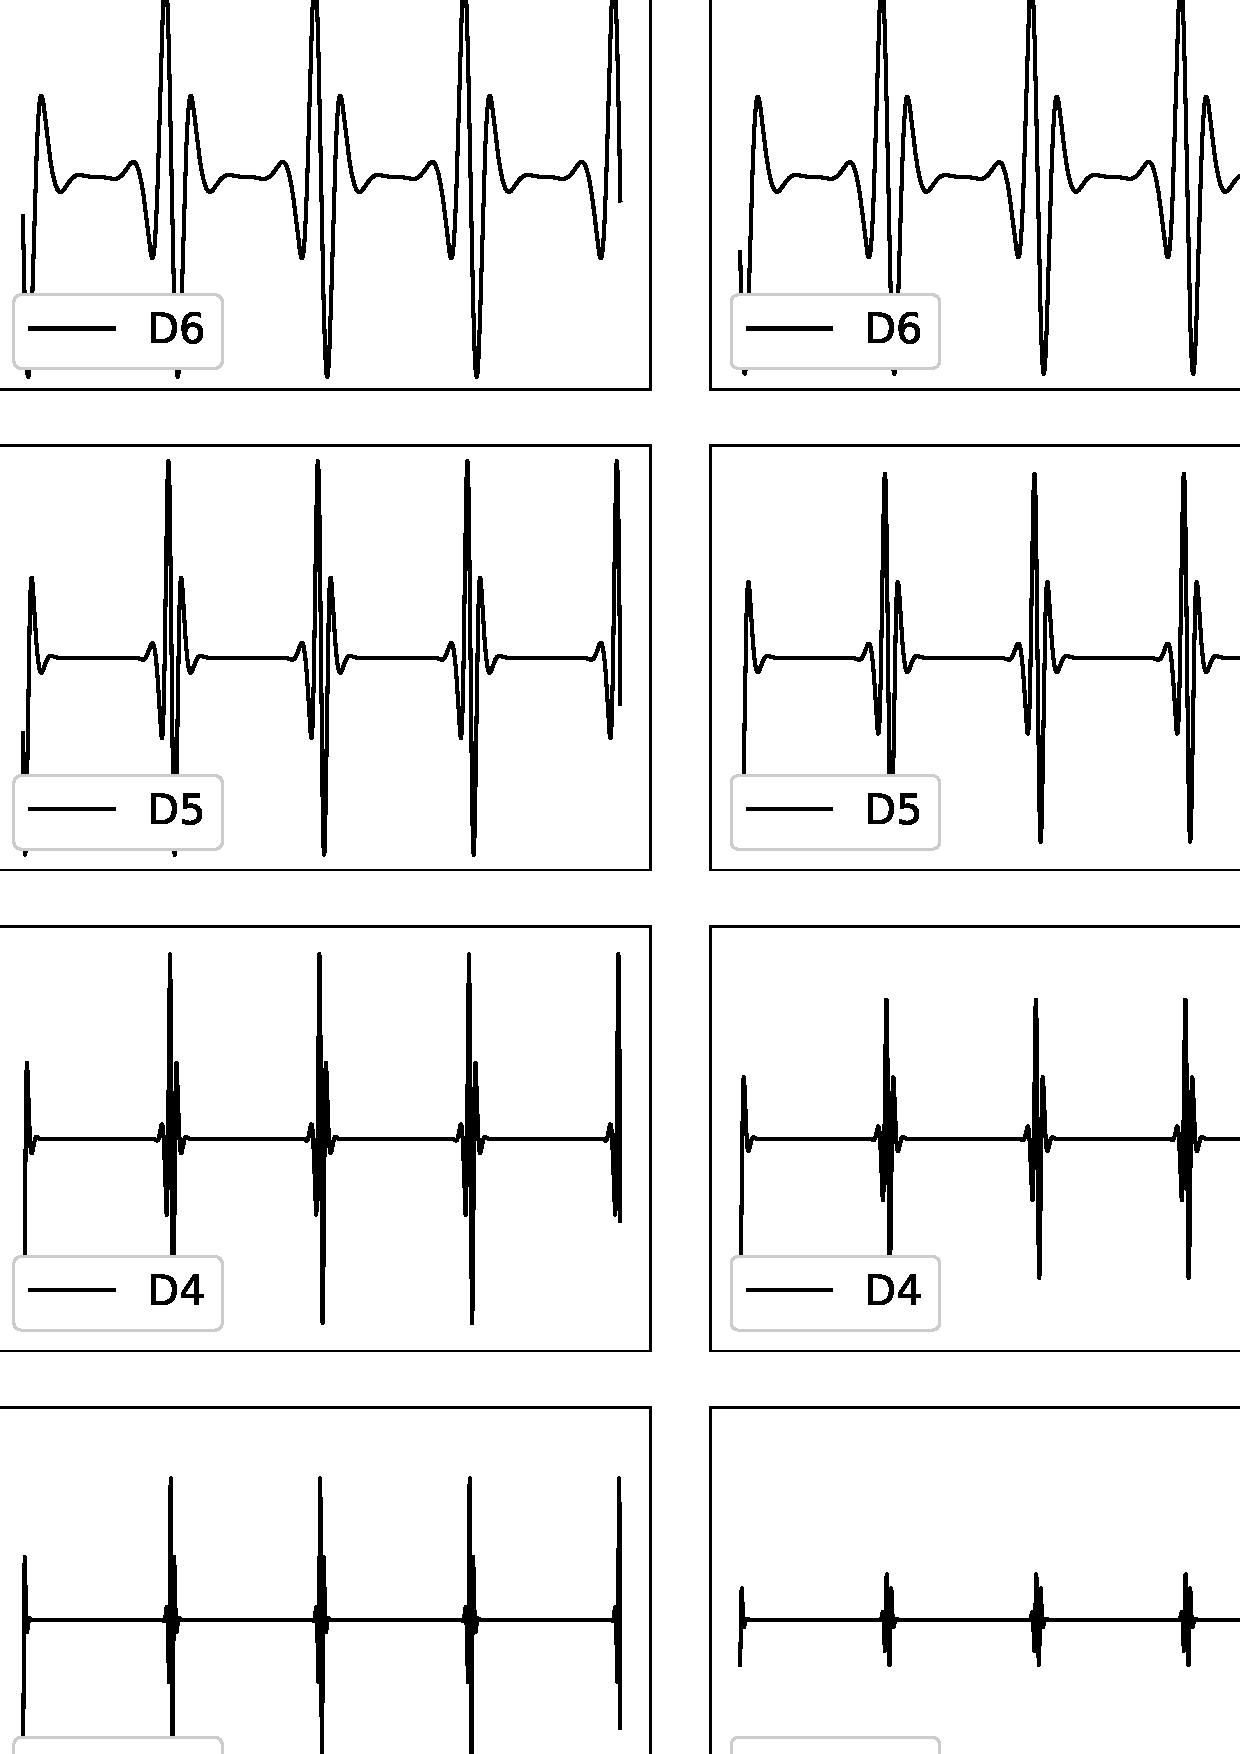
\includegraphics[width=\textwidth, trim={5cm 6cm 5cm 9cm},clip]{figures/500_DS.pdf}
\caption{Details and smooth of the wavelet decomposition of a synthetics signal with period 500 days and duration of the slow slip event equal to 2 days (left), 5 days, 10 days, and 20 days (right).}
\label{pngfiguresample}
\end{figure}

The ramp-like signal is transformed through the wavelet filtering into a waveform with first a positive peak and then a negative peak. The width of the waveform increases with the scale level. For the 8th level of the wavelet decomposition, the width of the waveform is nearly as large as the time between two events. We do not show details at larger scales as the corresponding waveforms would start to merge two contiguous events together, and make the wavelet decomposition less interpretable. For an event of duration 2 days, the wavelet details at levels higher than 2 have a larger amplitude than the wavelet detail at level 1. For an event of duration 5 days, the wavelet details at levels higher than 3 have a larger amplitude than the wavelet details at lower scales. For an event of duration 10 days, the wavelet details at levels higher than 5 have a larger amplitude than the wavelet details at lower scales. For an event of duration 20 days, the wavelet details at levels higher than 6 have a larger amplitude than the wavelet details at lower scales. Thus, the scale levels at which an event is being seen in the wavelet details give us an indication about the duration (and the magnitude) of the slow slip event. We expect the big slow slip events of magnitude 6-7 that lasts about 10 days to start being visible at the level 5 of the wavelet decomposition, but to not be noticeable at lower time scales. \\

\section{Results}

Explanation vespagram

Correlation

\section{Discussion}

\section{Conclusion}

%%

%  Numbered lines in equations:
%  To add line numbers to lines in equations,
%  \begin{linenomath*}
%  \begin{equation}
%  \end{equation}
%  \end{linenomath*}



%% Enter Figures and Tables near as possible to where they are first mentioned:
%
% DO NOT USE \psfrag or \subfigure commands.
%
% Figure captions go below the figure.
% Table titles go above tables;  other caption information
%  should be placed in last line of the table, using
% \multicolumn2l{$^a$ This is a table note.}
%
%----------------
% EXAMPLE FIGURE
%
% \begin{figure}[h]
% \centering
% when using pdflatex, use pdf file:
% \includegraphics[natwidth=800px,natheight=600px]{figsamp.pdf}
%
% when using dvips, use .eps file:
% \includegraphics[natwidth=800px,natheight=600px]{figsamp.eps}
%
% \caption{Short caption}
% \label{figone}
%  \end{figure}
%
% We recommend that you provide the native width and height (natwidth, natheight) of your figures.
% Specifying native dimensions ensures that your figures are properly scaled
%
%
% ---------------
% EXAMPLE TABLE
%
% \begin{table}
% \caption{Time of the Transition Between Phase 1 and Phase 2$^{a}$}
% \centering
% \begin{tabular}{l c}
% \hline
%  Run  & Time (min)  \\
% \hline
%   $l1$  & 260   \\
%   $l2$  & 300   \\
%   $l3$  & 340   \\
%   $h1$  & 270   \\
%   $h2$  & 250   \\
%   $h3$  & 380   \\
%   $r1$  & 370   \\
%   $r2$  & 390   \\
% \hline
% \multicolumn{2}{l}{$^{a}$Footnote text here.}
% \end{tabular}
% \end{table}

%% SIDEWAYS FIGURE and TABLE
% AGU prefers the use of {sidewaystable} over {landscapetable} as it causes fewer problems.
%
% \begin{sidewaysfigure}
% \includegraphics[width=20pc]{figsamp}
% \caption{caption here}
% \label{newfig}
% \end{sidewaysfigure}
%
%  \begin{sidewaystable}
%  \caption{Caption here}
% \label{tab:signif_gap_clos}
%  \begin{tabular}{ccc}
% one&two&three\\
% four&five&six
%  \end{tabular}
%  \end{sidewaystable}

%% If using numbered lines, please surround equations with \begin{linenomath*}...\end{linenomath*}
%\begin{linenomath*}
%\begin{equation}
%y|{f} \sim g(m, \sigma),
%\end{equation}
%\end{linenomath*}

%%% End of body of article

%%%%%%%%%%%%%%%%%%%%%%%%%%%%%%%%
%% Optional Appendix goes here
%
% The \appendix command resets counters and redefines section heads
%
% After typing \appendix
%
%\section{Here Is Appendix Title}
% will show
% A: Here Is Appendix Title
%
%\appendix
%\section{Here is a sample appendix}

%%%%%%%%%%%%%%%%%%%%%%%%%%%%%%%%%%%%%%%%%%%%%%%%%%%%%%%%%%%%%%%%
%
% Optional Glossary, Notation or Acronym section goes here:
%
%%%%%%%%%%%%%%
% Glossary is only allowed in Reviews of Geophysics
%  \begin{glossary}
%  \term{Term}
%   Term Definition here
%  \term{Term}
%   Term Definition here
%  \term{Term}
%   Term Definition here
%  \end{glossary}

%
%%%%%%%%%%%%%%
% Acronyms
%   \begin{acronyms}
%   \acro{Acronym}
%   Definition here
%   \acro{EMOS}
%   Ensemble model output statistics
%   \acro{ECMWF}
%   Centre for Medium-Range Weather Forecasts
%   \end{acronyms}

%
%%%%%%%%%%%%%%
% Notation
%   \begin{notation}
%   \notation{$a+b$} Notation Definition here
%   \notation{$e=mc^2$}
%   Equation in German-born physicist Albert Einstein's theory of special
%  relativity that showed that the increased relativistic mass ($m$) of a
%  body comes from the energy of motion of the body—that is, its kinetic
%  energy ($E$)—divided by the speed of light squared ($c^2$).
%   \end{notation}




%%%%%%%%%%%%%%%%%%%%%%%%%%%%%%%%%%%%%%%%%%%%%%%%%%%%%%%%%%%%%%%%
%
%  ACKNOWLEDGMENTS
%
% The acknowledgments must list:
%
% >>>>	A statement that indicates to the reader where the data
% 	supporting the conclusions can be obtained (for example, in the
% 	references, tables, supporting information, and other databases).
%
% 	All funding sources related to this work from all authors
%
% 	Any real or perceived financial conflicts of interests for any
%	author
%
% 	Other affiliations for any author that may be perceived as
% 	having a conflict of interest with respect to the results of this
% 	paper.
%
%
% It is also the appropriate place to thank colleagues and other contributors.
% AGU does not normally allow dedications.


\acknowledgments
Enter acknowledgments, including your data availability statement, here.


%% ------------------------------------------------------------------------ %%
%% References and Citations

%%%%%%%%%%%%%%%%%%%%%%%%%%%%%%%%%%%%%%%%%%%%%%%
% BibTeX is preferred:
%
% \bibliography{<name of your .bib file>}
%
% don't specify bibliographystyle
%%%%%%%%%%%%%%%%%%%%%%%%%%%%%%%%%%%%%%%%%%%%%%%



% Please use ONLY \citet and \citep for reference citations.
% DO NOT use other cite commands (e.g., \cite, \citeyear, \nocite, \citealp, etc.).
%% Example \citet and \citep:
%  ...as shown by \citet{Boug10}, \citet{Buiz07}, \citet{Fra10},
%  \citet{Ghel00}, and \citet{Leit74}.

%  ...as shown by \citep{Boug10}, \citep{Buiz07}, \citep{Fra10},
%  \citep{Ghel00, Leit74}.

%  ...has been shown \citep [e.g.,][]{Boug10,Buiz07,Fra10}.


\end{document}



More Information and Advice:

%% ------------------------------------------------------------------------ %%
%
%  SECTION HEADS
%
%% ------------------------------------------------------------------------ %%

% Capitalize the first letter of each word (except for
% prepositions, conjunctions, and articles that are
% three or fewer letters).

% AGU follows standard outline style; therefore, there cannot be a section 1 without
% a section 2, or a section 2.3.1 without a section 2.3.2.
% Please make sure your section numbers are balanced.
% ---------------
% Level 1 head
%
% Use the \section{} command to identify level 1 heads;
% type the appropriate head wording between the curly
% brackets, as shown below.
%
%An example:
%\section{Level 1 Head: Introduction}
%
% ---------------
% Level 2 head
%
% Use the \subsection{} command to identify level 2 heads.
%An example:
%\subsection{Level 2 Head}
%
% ---------------
% Level 3 head
%
% Use the \subsubsection{} command to identify level 3 heads
%An example:
%\subsubsection{Level 3 Head}
%
%---------------
% Level 4 head
%
% Use the \subsubsubsection{} command to identify level 3 heads
% An example:
%\subsubsubsection{Level 4 Head} An example.
%
%% ------------------------------------------------------------------------ %%
%
%  IN-TEXT LISTS
%
%% ------------------------------------------------------------------------ %%
%
% Do not use bulleted lists; enumerated lists are okay.
% \begin{enumerate}
% \item
% \item
% \item
% \end{enumerate}
%
%% ------------------------------------------------------------------------ %%
%
%  EQUATIONS
%
%% ------------------------------------------------------------------------ %%

% Single-line equations are centered.
% Equation arrays will appear left-aligned.

Math coded inside display math mode \[ ...\]
 will not be numbered, e.g.,:
 \[ x^2=y^2 + z^2\]

 Math coded inside \begin{equation} and \end{equation} will
 be automatically numbered, e.g.,:
 \begin{equation}
 x^2=y^2 + z^2
 \end{equation}


% To create multiline equations, use the
% \begin{eqnarray} and \end{eqnarray} environment
% as demonstrated below.
\begin{eqnarray}
  x_{1} & = & (x - x_{0}) \cos \Theta \nonumber \\
        && + (y - y_{0}) \sin \Theta  \nonumber \\
  y_{1} & = & -(x - x_{0}) \sin \Theta \nonumber \\
        && + (y - y_{0}) \cos \Theta.
\end{eqnarray}

%If you don't want an equation number, use the star form:
%\begin{eqnarray*}...\end{eqnarray*}

% Break each line at a sign of operation
% (+, -, etc.) if possible, with the sign of operation
% on the new line.

% Indent second and subsequent lines to align with
% the first character following the equal sign on the
% first line.

% Use an \hspace{} command to insert horizontal space
% into your equation if necessary. Place an appropriate
% unit of measure between the curly braces, e.g.
% \hspace{1in}; you may have to experiment to achieve
% the correct amount of space.


%% ------------------------------------------------------------------------ %%
%
%  EQUATION NUMBERING: COUNTER
%
%% ------------------------------------------------------------------------ %%

% You may change equation numbering by resetting
% the equation counter or by explicitly numbering
% an equation.

% To explicitly number an equation, type \eqnum{}
% (with the desired number between the brackets)
% after the \begin{equation} or \begin{eqnarray}
% command.  The \eqnum{} command will affect only
% the equation it appears with; LaTeX will number
% any equations appearing later in the manuscript
% according to the equation counter.
%

% If you have a multiline equation that needs only
% one equation number, use a \nonumber command in
% front of the double backslashes (\\) as shown in
% the multiline equation above.

% If you are using line numbers, remember to surround
% equations with \begin{linenomath*}...\end{linenomath*}

%  To add line numbers to lines in equations:
%  \begin{linenomath*}
%  \begin{equation}
%  \end{equation}
%  \end{linenomath*}



